% Taller 5 -- Lógica difusa. Compilar:
% tectonic -Z search-path=$HOME/repos/ud/maestria/mcic/.UniversidadDistrital-manual-marca/plantillas-latex informe_taller5.tex
% Las cifras salen de taller5_logica_difusa.ipynb ejecutado.
\documentclass[11pt,letterpaper]{article}
\usepackage{ud-informe}
\usepackage{amsmath}
\usepackage{qrcode}
\colorlet{udrojo}{udazul}
\definecolor{udrojoosc}{HTML}{0C6F96}

\renewcommand{\UDtitulo}{Clasificador difuso con reglas extraídas de datos}
\renewcommand{\UDsubtitulo}{Wine: funciones de pertenencia, t-normas, árbol de decisión y Fuzzy C-Means}
\renewcommand{\UDtipo}{Taller 5 -- Informe}
\renewcommand{\UDasignatura}{Inteligencia Computacional Aplicada}
\renewcommand{\UDdocente}{Cesar Andrey Perdomo Charry}
\renewcommand{\UDestudiantes}{Juan Felipe Rodríguez Galindo -- 20261595004}
\renewcommand{\UDencabezado}{Taller 5 -- Lógica difusa}

\begin{document}
\UDportada

\section{Introducción}

En este taller construí un clasificador difuso cuyas reglas salen directamente de los datos y lo probé en el conjunto Wine (178 vinos, 13 características químicas, 3 cultivares); para ello seguí el cuaderno \textit{Taller6B\_LogicaDifusa\_Propuesto\_Colab.ipynb} y resolví sus seis TODO: selección de 4 características sin fuga de información, la función de pertenencia sigmoidal, la fuerza de las reglas con las t-normas mínimo y producto, la evaluación con matriz de confusión, el experimento del número de etiquetas contra un árbol de decisión y el agrupamiento con Fuzzy C-Means, desarrollando solo la parte en Python; la parte en MATLAB (\textit{Taller\_Propuesto.mlx}) no la hice porque no tengo MATLAB, aunque el cuaderno deja exportados los dos CSV que esa parte usa.

Entregables: el cuaderno \texttt{taller5\_logica\_difusa.ipynb} ejecutado, \texttt{requirements.txt}, los archivos \texttt{wine\_4car\_train.csv} y \texttt{wine\_4car\_test.csv} que genera el cuaderno y este informe; antes de programar presenté el plan y mis hipótesis, quedando todo grabado en video (sección~\ref{sec:ia}).

\section{Marco teórico}

\textbf{Funciones de pertenencia.} Un conjunto difuso asigna a cada valor un grado entre 0 y 1, donde la triangular $\mathrm{trimf}(x;a,b,c)$ sube de 0 en $a$ a 1 en $b$ y baja a 0 en $c$; en contraste, la sigmoidal posee pendiente $a$ y cruce $c$:
\begin{equation*}
\mathrm{sigmf}(x;a,c)=\frac{1}{1+e^{-a(x-c)}},
\end{equation*}
vale 0,5 en $x=c$ y es estrictamente creciente si $a>0$, así que resulta apropiada para etiquetas abiertas como ``alto''.

\textbf{Reglas y t-normas.} Una regla adopta la forma ``SI $x_1$ es $A_1$ Y \dots{} Y $x_4$ es $A_4$ ENTONCES clase $= k$'', calculándose la conjunción con una t-norma sobre los grados de las cuatro condiciones, sea el mínimo, $\min_f \mu_{A_f}(x_f)$, o el producto, $\prod_f \mu_{A_f}(x_f)$. Dado que los grados yacen en $[0,1]$, siempre se cumple producto $\le$ mínimo; la muestra, por su parte, se asigna a la clase de la regla con mayor grado de disparo.

\textbf{Extracción de reglas (Wang-Mendel simplificado).} Cada característica se divide en $n_{mf}$ triangulares uniformes y para cada muestra de entrenamiento se toma la etiqueta de mayor grado en cada variable, conformando el antecedente mientras el consecuente corresponde a su clase. Si dos muestras producen antecedentes idénticos se conserva la de mayor grado, alcanzando con 4 características un tope teórico de $n_{mf}^4$ reglas.

\textbf{Fuzzy C-Means y ARI.} FCM agrupa sin recurrir a etiquetas: cada muestra pertenece a cada grupo con un grado, sumando 1 los grados de cada observación y minimizando con exponente $m=2$ la función $J=\sum_i\sum_k u_{ik}^m\,\lVert x_k-c_i\rVert^2$. El índice de Rand ajustado (ARI) contrasta el agrupamiento con las clases reales; vale 1 si coinciden plenamente y ronda 0 cuando el acuerdo equivale al azar, con la ventaja de no depender de cómo se numeren los grupos.

\section{Metodología}

\textbf{Entorno.} Se empleó Python 3.12 bajo un entorno de \texttt{uv} con numpy, matplotlib, scikit-learn y scikit-fuzzy (requiriendo networkx); las funciones de pertenencia, el clasificador y FCM fueron desarrollados directamente en el cuaderno, mientras scikit-fuzzy solo se utilizó para comprobar la sigmoidal. La semilla (\texttt{SEMILLA = 42}) y el conjunto (\texttt{DATASET = "wine"}) se fijan al inicio; cada TODO cuenta con un punto de control que reporta \texttt{[OK]} o \texttt{[REVISAR]}, quedando los 16 verificados en \texttt{[OK]}.

\textbf{Datos.} Se aplicó una partición estratificada 70-30 con semilla 42, asignando 124 vinos a entrenamiento (41, 50 y 33 por clase) y 54 a prueba (18, 21 y 15), ajustando \texttt{SelectKBest(f\_classif, k=4)} estrictamente sobre el entrenamiento. De haberse ajustado sobre la totalidad de los datos, las muestras de prueba habrían sesgado la selección hacia un desempeño optimista por fuga de información; así, las cuatro variables se normalizan a $[0,1]$ con los extremos del entrenamiento, recortando en prueba cualquier valor que desborde dicho rango.

\textbf{Experimentos.} Fijando $n_{mf}=3$ se extraen las reglas para comparar ambas t-normas (TODO 3), evaluando luego con producto la exactitud y la matriz de confusión (TODO 4); posteriormente, en el TODO 5 se varía $n_{mf}\in\{2,3,4\}$ contrastándolo con un \texttt{DecisionTreeClassifier} acotado en \texttt{max\_leaf\_nodes} al número de reglas extraídas sobre las mismas cuatro características. Finalmente, en el TODO 6, FCM agrupa los 178 vinos en $c=3$ conglomerados con $m=2$ prescindiendo de las etiquetas de clase para computar el ARI.

\section{Resultados}

\subsection{Características y t-normas (TODO 1 a 3)}

La tabla~\ref{tab:caracteristicas} muestra las cuatro características elegidas con su estadístico F en el entrenamiento.

\begin{table}[H]
\centering
\caption{Características elegidas por \texttt{SelectKBest} (ajustado solo con entrenamiento).}\label{tab:caracteristicas}
\begin{tabular}{lcc}
\toprule
Característica & F (ANOVA) & Rango en entrenamiento \\
\midrule
Flavonoides (\textit{flavanoids}) & 187,7 & 0,34 -- 3,74 \\
Prolina (\textit{proline}) & 149,4 & 278 -- 1515 \\
OD280/OD315 de vinos diluidos & 126,6 & 1,27 -- 3,92 \\
Alcohol & 100,3 & 11,03 -- 14,83 \\
\bottomrule
\end{tabular}
\end{table}

La sigmoidal superó los tres controles: vale 0,5 en $x=c$, es creciente con $a>0$ y coincide con \texttt{skfuzzy.sigmf}, que recibe los parámetros en el orden $(x, c, a)$; con $n_{mf}=3$ salieron 31 reglas de las 81 posibles (12 de la clase 0, 11 de la 1 y 8 de la 2), resumiéndose en la tabla~\ref{tab:tnormas} la comparación entre t-normas.

\begin{table}[H]
\centering
\caption{Clasificador difuso con $n_{mf}=3$ según la t-norma. La regla ganadora es la misma en los 54 vinos de prueba.}\label{tab:tnormas}
\begin{tabular}{lcc}
\toprule
T-norma & Reglas & Exactitud en prueba \\
\midrule
Producto & 31 & 92,6\,\% \\
Mínimo & 31 & 92,6\,\% \\
\bottomrule
\end{tabular}
\end{table}

\subsection{Evaluación con producto (TODO 4)}

La tabla~\ref{tab:confusion} corresponde a la matriz de confusión en prueba; se registran 4 errores en 54 vinos, donde el par más confundido corresponde a la clase 1 $\to$ clase 2 con 2 instancias.

\begin{table}[H]
\centering
\caption{Matriz de confusión en prueba ($n_{mf}=3$, producto).}\label{tab:confusion}
\begin{tabular}{lccc}
\toprule
Real $\backslash$ Predicha & Clase 0 & Clase 1 & Clase 2 \\
\midrule
Clase 0 & \textbf{17} & 1 & 0 \\
Clase 1 & 1 & \textbf{18} & 2 \\
Clase 2 & 0 & 0 & \textbf{15} \\
\bottomrule
\end{tabular}
\end{table}

Las tres reglas con mayor grado son:
\begin{enumerate}
\item SI alcohol es medio Y flavonoides es medio Y OD280/OD315 es medio Y prolina es media ENTONCES clase 1 (grado 0,60).
\item SI alcohol es bajo Y flavonoides es medio Y OD280/OD315 es medio Y prolina es baja ENTONCES clase 1 (grado 0,58).
\item SI alcohol es medio Y flavonoides es medio Y OD280/OD315 es medio Y prolina es baja ENTONCES clase 1 (grado 0,54).
\end{enumerate}

\subsection{Etiquetas contra árbol (TODO 5)}

La tabla~\ref{tab:nmf} y la figura~\ref{fig:nmf} muestran el experimento con 2, 3 y 4 etiquetas por característica.

\begin{table}[H]
\centering
\caption{Número de reglas y exactitud en prueba según $n_{mf}$. El árbol se limita a tantas hojas como reglas.}\label{tab:nmf}
\begin{tabular}{cccccc}
\toprule
$n_{mf}$ & Máximo ($n_{mf}^4$) & Reglas & Difuso & Hojas del árbol & Árbol \\
\midrule
2 & 16 & 10 & 75,9\,\% & 10 & 87,0\,\% \\
3 & 81 & 31 & 92,6\,\% & 13 & 87,0\,\% \\
4 & 256 & 43 & 88,9\,\% & 13 & 87,0\,\% \\
\bottomrule
\end{tabular}
\end{table}

\begin{figure}[H]
\centering
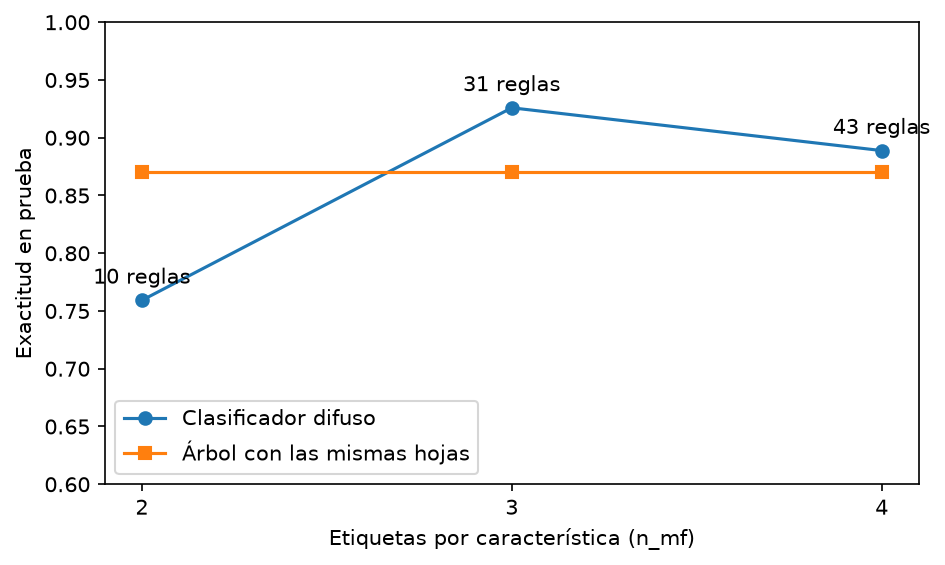
\includegraphics[width=0.75\linewidth]{../figuras/exactitud_nmf.png}
\caption{Exactitud en prueba del clasificador difuso y del árbol según el número de etiquetas.}\label{fig:nmf}
\end{figure}

\subsection{Fuzzy C-Means (TODO 6)}

FCM convergió en 19 iteraciones tras reducir $J$ de 15,7 a 7,4 y arrojando un ARI de 0,794 frente a las etiquetas reales. Al asignar cada vino al grupo de máxima pertenencia, cada conglomerado refleja predominantemente una clase: la clase 2 se agrupa íntegramente (48 de 48), la clase 0 casi en su totalidad (57 de 59) y la clase 1 en el tercero (60 de 71), quedando 10 vinos de la clase 1 dentro del grupo de la clase 2. El coeficiente de partición es 0,69, entre el valor de $1/3$ de una partición totalmente borrosa y el valor de 1 de una nítida.

\section{Análisis}

\textbf{Tres etiquetas es el punto medio.} Con 2 etiquetas cada variable solo discrimina entre ``bajo'' y ``alto'', de modo que 10 reglas resultan insuficientes para separar la clase 1, que queda en una franja intermedia en flavonoides y OD280/OD315, lo cual degrada la exactitud al 75,9\,\%; en cambio, con 4 etiquetas se generan 43 reglas donde muchas provienen de un único vino de entrenamiento sin repetirse en prueba (incluso una muestra de prueba queda sin regla activa), cayendo la exactitud a 88,9\,\%.

\textbf{Hay muchas menos reglas que combinaciones.} Las reglas se manifiestan únicamente donde existen datos: con 3 etiquetas aparecen 31 de 81 antecedentes y con 4 apenas 43 de 256; esto ocurre porque varias características están correlacionadas (flavonoides con OD280/OD315, 0,77; alcohol con prolina, 0,66), de modo que muchas combinaciones de etiquetas nunca se presentan en los datos.

\textbf{El árbol no cambia.} Con 10 hojas el árbol alcanza 87,0\,\%, pero al autorizarle 31 o 43 hojas utiliza únicamente 13, puesto que a esa profundidad todas las hojas son homogéneas en entrenamiento y carece de impureza por escindir; por este motivo su exactitud permanece fija en 87,0\,\% a partir de $n_{mf}=3$, volviendo inocuo el techo de hojas.

\textbf{Mínimo y producto coinciden.} Aunque el producto genera grados sistemáticamente menores o iguales al mínimo, la decisión final depende exclusivamente de la regla dominante; en los 54 vinos de prueba la regla ganadora coincide bajo ambas t-normas, derivando en una exactitud idéntica.

\textbf{Los errores son esperables.} Tres de los cuatro fallos son vinos de la clase 1, que queda entre las otras dos en flavonoides y OD280/OD315 y se parece a la clase 2 en alcohol y prolina (medias de 12,24 frente a 13,07 y de 531 frente a 624), patrón que FCM replica de forma no supervisada al ser la clase 1 la que se bifurca entre dos grupos.

\textbf{La muestra de prueba es pequeña.} Al contar con 54 vinos cada observación representa 1,85 puntos porcentuales, de modo que la brecha entre 92,6\,\% y 88,9\,\% obedece a apenas 2 vinos y entre 92,6\,\% y 87,0\,\% a 3, por lo que una partición distinta podría alterar dicho escalonamiento.

\textbf{Hipótesis contra resultados.} Antes de ejecutar escribí cuatro hipótesis en la presentación del plan:
\begin{enumerate}
\item \textit{``Con más etiquetas habrá más reglas y al principio funcionará mejor, pero se sobreentrenará.''} Se cumplió: las reglas crecen (10, 31, 43) y la exactitud sube de 2 a 3 etiquetas y baja con 4.
\item \textit{``En algunos casos más etiquetas degradarán la exactitud.''} Se cumplió: de 3 a 4 etiquetas bajó de 92,6\,\% a 88,9\,\%.
\item \textit{``Casi no cambia la regla ganadora, así que la exactitud será parecida.''} Se cumplió del todo: la regla ganadora es la misma en los 54 vinos.
\item \textit{``El árbol se puede complejizar hasta desempeñarse mejor que el difuso.''} Se cumplió solo con 2 etiquetas (87,0\,\% contra 75,9\,\%); con 3 y 4 el árbol se estanca al saturar la pureza de sus hojas y el difuso lo supera.
\end{enumerate}

\textbf{Interpretabilidad.} Las reglas difusas se formulan de manera natural en términos del dominio (``alcohol medio y prolina baja''), especificando el grado de pertenencia con el que disparan; si bien el árbol también resulta legible, sus particiones trazan fronteras rígidas donde una pequeña variación desplaza la muestra de rama, mientras el enfoque difuso modula gradualmente su pertenencia compartida.

\section{Conclusiones}

\begin{enumerate}
\item La selección sin fuga ajustada en entrenamiento aisló flavonoides, prolina, OD280/OD315 y alcohol como las variables más discriminantes según el estadístico F.
\item Con 3 etiquetas por variable, Wang-Mendel extrajo 31 reglas y clasificó correctamente el 92,6\,\% del conjunto de prueba (50 de 54 vinos), arrojando igual exactitud con mínimo y producto al no variar la regla ganadora.
\item La principal confusión se produjo en la transición clase 1 $\to$ clase 2 (2 vinos), explicada porque la clase 1 se parece a la clase 2 en alcohol y prolina y queda entre las otras dos en flavonoides y OD280/OD315.
\item Incrementar etiquetas no garantiza mejoría: ante 2, 3 y 4 etiquetas la exactitud fue 75,9\,\%, 92,6\,\% y 88,9\,\%, mientras el árbol se limitó a 87,0\,\% al copar 13 hojas puras.
\item De modo no supervisado, Fuzzy C-Means reconstruyó los tres cultivares con un ARI de 0,794, reproduciendo la misma ambigüedad entre las clases 1 y 2.
\end{enumerate}

\section{Declaración de uso de IA}\label{sec:ia}

Usé Claude (Anthropic) para revisar y corregir errores y para redactar este informe a partir de los resultados del cuaderno. Todo el desarrollo quedó grabado (cerca de 1 hora y 15 minutos):

\begin{center}
\qrcode[height=3.2cm,nolink]{https://youtu.be/sCQziT3QukI}\\[0.6em]
\url{https://youtu.be/sCQziT3QukI}
\end{center}

\end{document}
